% Options for packages loaded elsewhere
\PassOptionsToPackage{unicode}{hyperref}
\PassOptionsToPackage{hyphens}{url}
%
\documentclass[
]{article}
\usepackage{amsmath,amssymb}
\usepackage{lmodern}
\usepackage{iftex}
\ifPDFTeX
  \usepackage[T1]{fontenc}
  \usepackage[utf8]{inputenc}
  \usepackage{textcomp} % provide euro and other symbols
\else % if luatex or xetex
  \usepackage{unicode-math}
  \defaultfontfeatures{Scale=MatchLowercase}
  \defaultfontfeatures[\rmfamily]{Ligatures=TeX,Scale=1}
\fi
% Use upquote if available, for straight quotes in verbatim environments
\IfFileExists{upquote.sty}{\usepackage{upquote}}{}
\IfFileExists{microtype.sty}{% use microtype if available
  \usepackage[]{microtype}
  \UseMicrotypeSet[protrusion]{basicmath} % disable protrusion for tt fonts
}{}
\makeatletter
\@ifundefined{KOMAClassName}{% if non-KOMA class
  \IfFileExists{parskip.sty}{%
    \usepackage{parskip}
  }{% else
    \setlength{\parindent}{0pt}
    \setlength{\parskip}{6pt plus 2pt minus 1pt}}
}{% if KOMA class
  \KOMAoptions{parskip=half}}
\makeatother
\usepackage{xcolor}
\IfFileExists{xurl.sty}{\usepackage{xurl}}{} % add URL line breaks if available
\IfFileExists{bookmark.sty}{\usepackage{bookmark}}{\usepackage{hyperref}}
\hypersetup{
  pdftitle={Harmonicity in early auditory processing - power analysis},
  pdfauthor={Krzysztof Basiński (based on a script by David Quiroga)},
  hidelinks,
  pdfcreator={LaTeX via pandoc}}
\urlstyle{same} % disable monospaced font for URLs
\usepackage[margin=1in]{geometry}
\usepackage{color}
\usepackage{fancyvrb}
\newcommand{\VerbBar}{|}
\newcommand{\VERB}{\Verb[commandchars=\\\{\}]}
\DefineVerbatimEnvironment{Highlighting}{Verbatim}{commandchars=\\\{\}}
% Add ',fontsize=\small' for more characters per line
\usepackage{framed}
\definecolor{shadecolor}{RGB}{248,248,248}
\newenvironment{Shaded}{\begin{snugshade}}{\end{snugshade}}
\newcommand{\AlertTok}[1]{\textcolor[rgb]{0.94,0.16,0.16}{#1}}
\newcommand{\AnnotationTok}[1]{\textcolor[rgb]{0.56,0.35,0.01}{\textbf{\textit{#1}}}}
\newcommand{\AttributeTok}[1]{\textcolor[rgb]{0.77,0.63,0.00}{#1}}
\newcommand{\BaseNTok}[1]{\textcolor[rgb]{0.00,0.00,0.81}{#1}}
\newcommand{\BuiltInTok}[1]{#1}
\newcommand{\CharTok}[1]{\textcolor[rgb]{0.31,0.60,0.02}{#1}}
\newcommand{\CommentTok}[1]{\textcolor[rgb]{0.56,0.35,0.01}{\textit{#1}}}
\newcommand{\CommentVarTok}[1]{\textcolor[rgb]{0.56,0.35,0.01}{\textbf{\textit{#1}}}}
\newcommand{\ConstantTok}[1]{\textcolor[rgb]{0.00,0.00,0.00}{#1}}
\newcommand{\ControlFlowTok}[1]{\textcolor[rgb]{0.13,0.29,0.53}{\textbf{#1}}}
\newcommand{\DataTypeTok}[1]{\textcolor[rgb]{0.13,0.29,0.53}{#1}}
\newcommand{\DecValTok}[1]{\textcolor[rgb]{0.00,0.00,0.81}{#1}}
\newcommand{\DocumentationTok}[1]{\textcolor[rgb]{0.56,0.35,0.01}{\textbf{\textit{#1}}}}
\newcommand{\ErrorTok}[1]{\textcolor[rgb]{0.64,0.00,0.00}{\textbf{#1}}}
\newcommand{\ExtensionTok}[1]{#1}
\newcommand{\FloatTok}[1]{\textcolor[rgb]{0.00,0.00,0.81}{#1}}
\newcommand{\FunctionTok}[1]{\textcolor[rgb]{0.00,0.00,0.00}{#1}}
\newcommand{\ImportTok}[1]{#1}
\newcommand{\InformationTok}[1]{\textcolor[rgb]{0.56,0.35,0.01}{\textbf{\textit{#1}}}}
\newcommand{\KeywordTok}[1]{\textcolor[rgb]{0.13,0.29,0.53}{\textbf{#1}}}
\newcommand{\NormalTok}[1]{#1}
\newcommand{\OperatorTok}[1]{\textcolor[rgb]{0.81,0.36,0.00}{\textbf{#1}}}
\newcommand{\OtherTok}[1]{\textcolor[rgb]{0.56,0.35,0.01}{#1}}
\newcommand{\PreprocessorTok}[1]{\textcolor[rgb]{0.56,0.35,0.01}{\textit{#1}}}
\newcommand{\RegionMarkerTok}[1]{#1}
\newcommand{\SpecialCharTok}[1]{\textcolor[rgb]{0.00,0.00,0.00}{#1}}
\newcommand{\SpecialStringTok}[1]{\textcolor[rgb]{0.31,0.60,0.02}{#1}}
\newcommand{\StringTok}[1]{\textcolor[rgb]{0.31,0.60,0.02}{#1}}
\newcommand{\VariableTok}[1]{\textcolor[rgb]{0.00,0.00,0.00}{#1}}
\newcommand{\VerbatimStringTok}[1]{\textcolor[rgb]{0.31,0.60,0.02}{#1}}
\newcommand{\WarningTok}[1]{\textcolor[rgb]{0.56,0.35,0.01}{\textbf{\textit{#1}}}}
\usepackage{graphicx}
\makeatletter
\def\maxwidth{\ifdim\Gin@nat@width>\linewidth\linewidth\else\Gin@nat@width\fi}
\def\maxheight{\ifdim\Gin@nat@height>\textheight\textheight\else\Gin@nat@height\fi}
\makeatother
% Scale images if necessary, so that they will not overflow the page
% margins by default, and it is still possible to overwrite the defaults
% using explicit options in \includegraphics[width, height, ...]{}
\setkeys{Gin}{width=\maxwidth,height=\maxheight,keepaspectratio}
% Set default figure placement to htbp
\makeatletter
\def\fps@figure{htbp}
\makeatother
\setlength{\emergencystretch}{3em} % prevent overfull lines
\providecommand{\tightlist}{%
  \setlength{\itemsep}{0pt}\setlength{\parskip}{0pt}}
\setcounter{secnumdepth}{-\maxdimen} % remove section numbering
\ifLuaTeX
  \usepackage{selnolig}  % disable illegal ligatures
\fi

\title{Harmonicity in early auditory processing - power analysis}
\author{Krzysztof Basiński (based on a script by David Quiroga)}
\date{2022-03-16}

\begin{document}
\maketitle

First, load the \emph{lme4} library and define a function to conduct
power estimates.

\begin{Shaded}
\begin{Highlighting}[]
\FunctionTok{library}\NormalTok{(lme4)}
\end{Highlighting}
\end{Shaded}

\begin{verbatim}
## Loading required package: Matrix
\end{verbatim}

\begin{Shaded}
\begin{Highlighting}[]
\NormalTok{pwr\_calc }\OtherTok{\textless{}{-}} \ControlFlowTok{function}\NormalTok{(b0,b1,b0\_sd,res\_sd,nsims,ssizes) \{}
  \CommentTok{\# intialize data frame to store the output }
\NormalTok{  pwr }\OtherTok{\textless{}{-}} \FunctionTok{data.frame}\NormalTok{() }
  
  \ControlFlowTok{for}\NormalTok{ (s }\ControlFlowTok{in} \DecValTok{1}\SpecialCharTok{:}\FunctionTok{length}\NormalTok{(ssizes)) \{}
    \ControlFlowTok{for}\NormalTok{ (n }\ControlFlowTok{in} \DecValTok{1}\SpecialCharTok{:}\NormalTok{nsims) \{}
      \CommentTok{\# df index}
\NormalTok{      idx }\OtherTok{\textless{}{-}}\NormalTok{ (s}\DecValTok{{-}1}\NormalTok{) }\SpecialCharTok{*}\NormalTok{ nsims }\SpecialCharTok{+}\NormalTok{ n}
      
      \CommentTok{\# current sample size}
\NormalTok{      ssize }\OtherTok{\textless{}{-}}\NormalTok{ ssizes[s]}
      
      \CommentTok{\# conditions factor}
\NormalTok{      conds }\OtherTok{\textless{}{-}} \FunctionTok{rep}\NormalTok{(}\FunctionTok{c}\NormalTok{(}\DecValTok{0}\NormalTok{,}\DecValTok{1}\NormalTok{,}\DecValTok{2}\NormalTok{),ssize)}
      
      \CommentTok{\# subject id\textquotesingle{}s}
\NormalTok{      subs }\OtherTok{\textless{}{-}} \FunctionTok{rep}\NormalTok{(}\DecValTok{1}\SpecialCharTok{:}\NormalTok{ssize, }\AttributeTok{each =} \FunctionTok{length}\NormalTok{(}\FunctionTok{unique}\NormalTok{(conds)))}
      
      \CommentTok{\# add intercept}
\NormalTok{      intercept }\OtherTok{\textless{}{-}} \FunctionTok{rep}\NormalTok{(}\FunctionTok{rnorm}\NormalTok{(ssize,b0,b0\_sd), }\AttributeTok{each =} \FunctionTok{length}\NormalTok{(}\FunctionTok{unique}\NormalTok{(conds)))}
      
      \CommentTok{\# add condition effect}
\NormalTok{      conds\_effect }\OtherTok{\textless{}{-}} \FunctionTok{rep}\NormalTok{(}\FunctionTok{c}\NormalTok{(}\DecValTok{0}\NormalTok{,}\DecValTok{0}\NormalTok{,}\DecValTok{1}\NormalTok{),ssize)}
\NormalTok{      beta1 }\OtherTok{\textless{}{-}} \FunctionTok{rep}\NormalTok{(b1,}\AttributeTok{each=} \FunctionTok{length}\NormalTok{(}\FunctionTok{unique}\NormalTok{(conds)))}\SpecialCharTok{*}\NormalTok{conds\_effect}
      
      \CommentTok{\# add residual noise}
\NormalTok{      residuals }\OtherTok{\textless{}{-}} \FunctionTok{rnorm}\NormalTok{(}\FunctionTok{length}\NormalTok{(subs),}\DecValTok{0}\NormalTok{,res\_sd)}
      
      \CommentTok{\# collect in a dataframe and calculate simulated measured outcome (y)}
\NormalTok{      d }\OtherTok{\textless{}{-}} \FunctionTok{data.frame}\NormalTok{(}\StringTok{\textquotesingle{}cond\textquotesingle{}} \OtherTok{=} \FunctionTok{as.character}\NormalTok{(conds), }
                      \StringTok{\textquotesingle{}sub\textquotesingle{}} \OtherTok{=}\NormalTok{ subs,}
                      \StringTok{\textquotesingle{}b0\textquotesingle{}} \OtherTok{=}\NormalTok{ intercept,}
                      \StringTok{\textquotesingle{}b1\textquotesingle{}} \OtherTok{=}\NormalTok{ beta1,}
                      \StringTok{\textquotesingle{}res\textquotesingle{}} \OtherTok{=}\NormalTok{ residuals,}
                      \StringTok{\textquotesingle{}y\textquotesingle{}} \OtherTok{=}\NormalTok{ intercept }\SpecialCharTok{+}\NormalTok{ beta1 }\SpecialCharTok{+}\NormalTok{ residuals)}
      
      \CommentTok{\# fit models}
\NormalTok{      m0 }\OtherTok{\textless{}{-}} \FunctionTok{lmer}\NormalTok{(y}\SpecialCharTok{\textasciitilde{}}\DecValTok{1} \SpecialCharTok{+}\NormalTok{ (}\DecValTok{1}\SpecialCharTok{|}\NormalTok{sub), }\AttributeTok{data =}\NormalTok{ d, }\AttributeTok{REML =} \ConstantTok{FALSE}\NormalTok{)}
\NormalTok{      m1 }\OtherTok{\textless{}{-}} \FunctionTok{lmer}\NormalTok{(y}\SpecialCharTok{\textasciitilde{}}\NormalTok{cond }\SpecialCharTok{+}\NormalTok{ (}\DecValTok{1}\SpecialCharTok{|}\NormalTok{sub), }\AttributeTok{data =}\NormalTok{ d, }\AttributeTok{REML =} \ConstantTok{FALSE}\NormalTok{)}
      
      \CommentTok{\# perform likelihood ratio test}
\NormalTok{      test }\OtherTok{\textless{}{-}} \FunctionTok{anova}\NormalTok{(m0,m1)}
      
      \CommentTok{\#store output of simulation}
\NormalTok{      pwr[idx,}\StringTok{\textquotesingle{}sim\textquotesingle{}}\NormalTok{] }\OtherTok{\textless{}{-}}\NormalTok{ n}
\NormalTok{      pwr[idx, }\StringTok{\textquotesingle{}ssize\textquotesingle{}}\NormalTok{] }\OtherTok{\textless{}{-}}\NormalTok{ ssize}
\NormalTok{      pwr[idx, }\StringTok{\textquotesingle{}b0\textquotesingle{}}\NormalTok{] }\OtherTok{\textless{}{-}} \FunctionTok{summary}\NormalTok{(m1)}\SpecialCharTok{$}\NormalTok{coefficients[}\DecValTok{1}\NormalTok{]}
\NormalTok{      pwr[idx, }\StringTok{\textquotesingle{}b1\textquotesingle{}}\NormalTok{] }\OtherTok{\textless{}{-}} \FunctionTok{summary}\NormalTok{(m1)}\SpecialCharTok{$}\NormalTok{coefficients[}\DecValTok{2}\NormalTok{]}
\NormalTok{      pwr[idx, }\StringTok{\textquotesingle{}sd\_int\textquotesingle{}}\NormalTok{] }\OtherTok{\textless{}{-}} \FunctionTok{attr}\NormalTok{(}\FunctionTok{summary}\NormalTok{(m1)}\SpecialCharTok{$}\NormalTok{varcor}\SpecialCharTok{$}\NormalTok{sub,}\StringTok{"stddev"}\NormalTok{) }
\NormalTok{      pwr[idx, }\StringTok{\textquotesingle{}sd\_res\textquotesingle{}}\NormalTok{] }\OtherTok{\textless{}{-}} \FunctionTok{summary}\NormalTok{(m1)}\SpecialCharTok{$}\NormalTok{sigma}
\NormalTok{      pwr[idx, }\StringTok{\textquotesingle{}x2\textquotesingle{}}\NormalTok{] }\OtherTok{\textless{}{-}}\NormalTok{ test}\SpecialCharTok{$}\NormalTok{Chisq[}\DecValTok{2}\NormalTok{]}
\NormalTok{      pwr[idx, }\StringTok{\textquotesingle{}p\textquotesingle{}}\NormalTok{] }\OtherTok{\textless{}{-}}\NormalTok{ test}\SpecialCharTok{$}\StringTok{\textasciigrave{}}\AttributeTok{Pr(\textgreater{}Chisq)}\StringTok{\textasciigrave{}}\NormalTok{[}\DecValTok{2}\NormalTok{]}
\NormalTok{    \}}
\NormalTok{  \}}
  \FunctionTok{return}\NormalTok{(pwr)}
\NormalTok{\}}
\end{Highlighting}
\end{Shaded}

This function uses a mixed effects modelling to compare a null model in
the form:

\texttt{y\ \textasciitilde{}\ 1\ +\ (1\ \textbar{}\ participant)}

to the model:

\texttt{y\ \textasciitilde{}\ harmonicity\ +\ (1\ \textbar{}\ participant)}

Where \texttt{y} is the dependent variable (EEG results), harmonicity is
a fixed effect and participant is a random effect. Harmonicity is
specified as a three-level factor (harmonic, inharmonic, inharmonic
changing).

Now specify the parameters to simulate EEG data. Let's assume a minimum
difference of -1uV (micro volts) between the harmonic and inharmonic
conditions and a residual SD of 1.5uV. Let's also assume a `worst case'
scenario, where there are no detectable differences between inharmonic
and inharmonic-changing conditions. This script runs 10 000 simulations
for each possible sample size from N = 25 to N = 40.

\begin{Shaded}
\begin{Highlighting}[]
\NormalTok{e0 }\OtherTok{\textless{}{-}} \DecValTok{3} \CommentTok{\# uV \# uV \# intercept (in fT or micro Volts)}
\NormalTok{e1 }\OtherTok{\textless{}{-}} \SpecialCharTok{{-}}\DecValTok{1} \CommentTok{\# {-}1 uv \# uV \# minimum difference between conditions}
\NormalTok{e0\_sd }\OtherTok{\textless{}{-}} \FloatTok{0.95} \CommentTok{\# 0.95 uV \# standard deviation of the intercept }
\NormalTok{eres\_sd }\OtherTok{\textless{}{-}} \FloatTok{1.5} \CommentTok{\# 1.5 uV \# residual standard deviation}
\NormalTok{nsims }\OtherTok{\textless{}{-}} \DecValTok{10000} \CommentTok{\# number of simulations per sample size}
\NormalTok{ssizes }\OtherTok{\textless{}{-}} \FunctionTok{seq}\NormalTok{(}\AttributeTok{from =} \DecValTok{25}\NormalTok{, }\AttributeTok{to =} \DecValTok{40}\NormalTok{, }\AttributeTok{by =} \DecValTok{1}\NormalTok{) }\CommentTok{\# sample sizes}

\FunctionTok{set.seed}\NormalTok{(}\DecValTok{777}\NormalTok{)}
\NormalTok{pwr2 }\OtherTok{\textless{}{-}} \FunctionTok{pwr\_calc}\NormalTok{(e0,e1,e0\_sd,eres\_sd,nsims,ssizes)}



\NormalTok{summary2 }\OtherTok{\textless{}{-}} \FunctionTok{aggregate}\NormalTok{(pwr2}\SpecialCharTok{$}\NormalTok{p,}\AttributeTok{by =} \FunctionTok{list}\NormalTok{(pwr2}\SpecialCharTok{$}\NormalTok{ssize), }\AttributeTok{FUN =} \ControlFlowTok{function}\NormalTok{(x) }\FunctionTok{sum}\NormalTok{(x }\SpecialCharTok{\textless{}} \FloatTok{0.05}\NormalTok{)}\SpecialCharTok{/}\FunctionTok{length}\NormalTok{(x))}
\FunctionTok{colnames}\NormalTok{(summary2) }\OtherTok{\textless{}{-}} \FunctionTok{c}\NormalTok{(}\StringTok{\textquotesingle{}sample.size\textquotesingle{}}\NormalTok{,}\StringTok{\textquotesingle{}power\textquotesingle{}}\NormalTok{)}
\FunctionTok{print}\NormalTok{(summary2)}
\end{Highlighting}
\end{Shaded}

\begin{verbatim}
##    sample.size  power
## 1           25 0.6640
## 2           26 0.6965
## 3           27 0.7015
## 4           28 0.7280
## 5           29 0.7353
## 6           30 0.7562
## 7           31 0.7693
## 8           32 0.7804
## 9           33 0.8034
## 10          34 0.8109
## 11          35 0.8242
## 12          36 0.8303
## 13          37 0.8461
## 14          38 0.8569
## 15          39 0.8661
## 16          40 0.8707
\end{verbatim}

Now plot the power curve as a function of sample size:

\begin{Shaded}
\begin{Highlighting}[]
\FunctionTok{with}\NormalTok{(summary2, }\FunctionTok{plot}\NormalTok{(sample.size, power, }\AttributeTok{type =} \StringTok{\textquotesingle{}ol\textquotesingle{}}\NormalTok{)) }
\FunctionTok{abline}\NormalTok{(}\AttributeTok{h=}\NormalTok{.}\DecValTok{8}\NormalTok{, }\AttributeTok{col=}\StringTok{\textquotesingle{}red\textquotesingle{}}\NormalTok{)}
\FunctionTok{title}\NormalTok{(}\StringTok{\textquotesingle{}Power curve\textquotesingle{}}\NormalTok{)}
\end{Highlighting}
\end{Shaded}

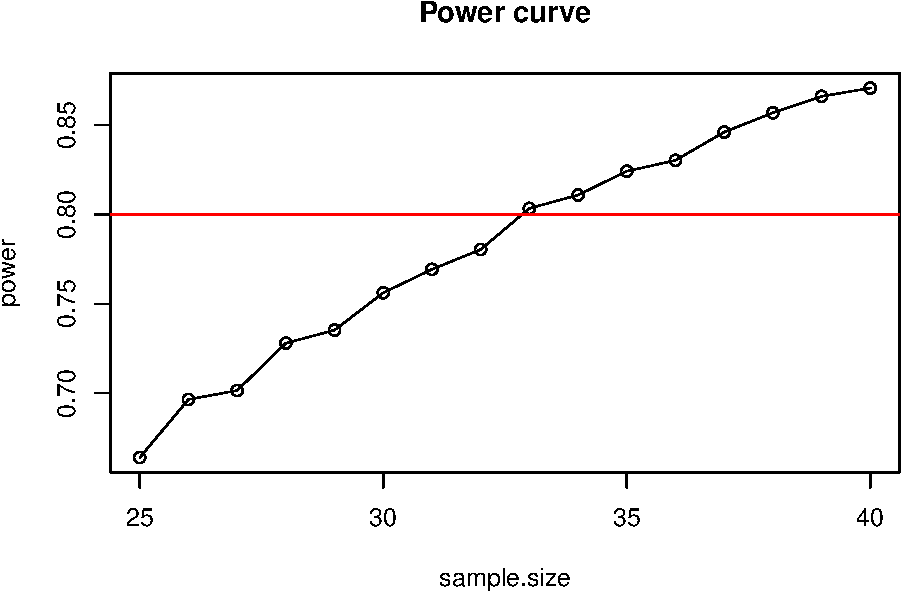
\includegraphics{power_analysis-0-5_files/figure-latex/unnamed-chunk-3-1.pdf}

This analysis shows that a power level of 0.8 is achieved for a sample
size of N = 33.

\end{document}
